\subsection{Расчёт циклона}
\label{cycRes}
\paragraph{Постановка задачи\\}
\addcontentsline{toc}{paragraph}{Постановка задачи}
В задаче рассматривается турбулентное течение вязкого газа с дисперсными включениями в циклоне модели Stairmand c учётом влияния дисперсной фазы на исходное течение. Геометрические параметры циклона представлены в \textit{таблице \ref{cycloneGeomPar}}.

  \begin{minipage}{0.6\textwidth}
    \captionof{table}{Геометрия фильтра}
    \label{cycloneGeomPar}
			\begin{tabular}{l l}
				\hline
				\label{geometrytable}
				Диаметр цилиндра, $D$ & $0.205m$ \\
				Диаметр выходной трубы, $D_e$ & $0.5D$ \\
				Высота входного канала, $a$ & $0.5D$ \\
				Ширина входного канала, $b$ & $0.2D$ \\
				Длина выходной трубы, $h_e$ & $0.75D$ \\
				Полная высота фильтра, $H$ & $4.0D$ \\
				Высота цилиндра, $h$ & $1.5D$ \\
				Диаметр нижнего сечения, $B$ & $0.36D$ \\
				Высота пылесборника, $h_d$ & $0.25D$ \\
				Диаметр пылесборника, $D_d$ & $0.75D$ \\
			\end{tabular}
    \end{minipage}
    \hspace{1em}
  \begin{minipage}{0.35\textwidth}
    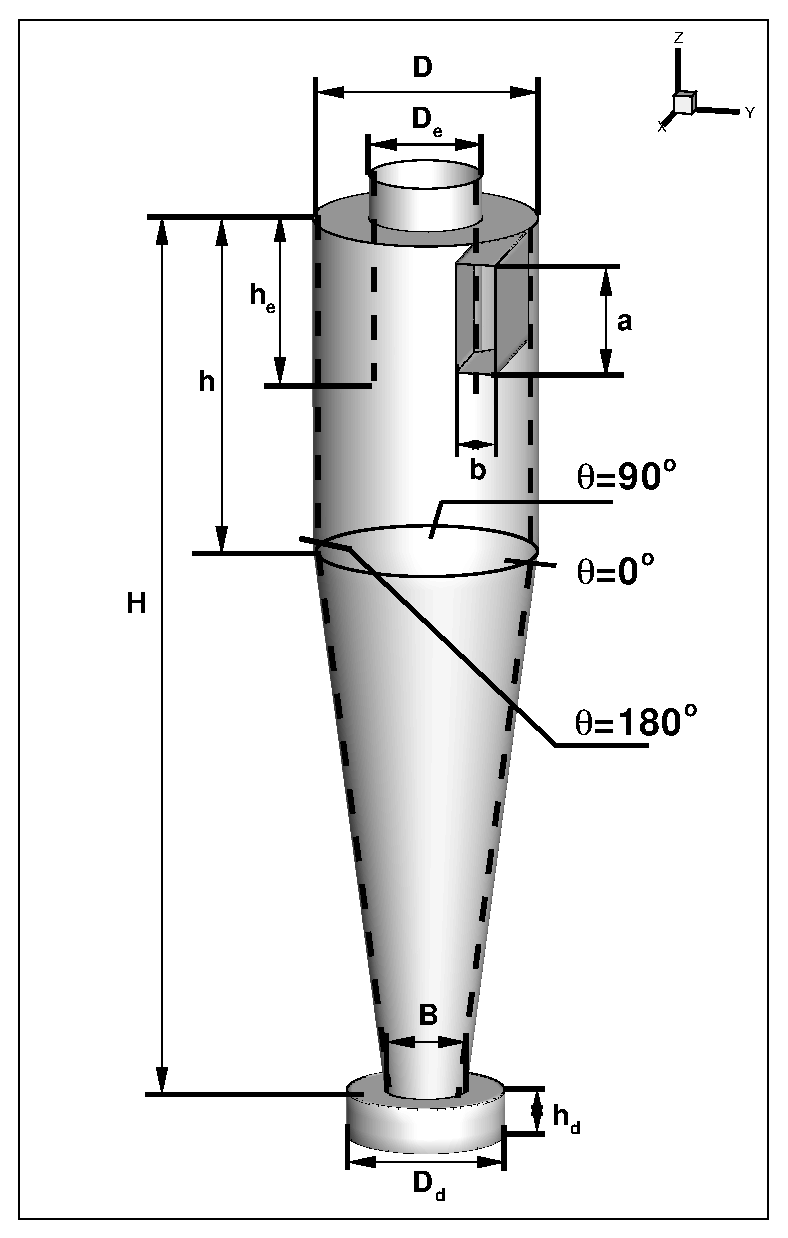
\includegraphics[scale=0.45]{cycloneGeometryTeta}
	\captionof{figure}{Схема фильтра}
	\label{fig:cycloneGeometryScheme}
  \end{minipage}
  \vspace{1em}
	
	Течение исследуется для 4 различных скоростей на входе, а также для трёх разных порядков величины диаметра частиц. Граничные условия для задачи описаны в \textit{таблице \ref{cycloneBC}}, а на \textit{рисунке \ref{fig:cycloneMesh}} показана сетка расчётной области.
	
\begin{minipage}{0.6\textwidth}
    \captionof{table}{Граничные условия}
    \label{cycloneBC}
	\begin{tabular}{c}
		\hline
		\label{geometrytable}
		Скорость на входе, $U_{in}=$  $5, 10, 15, 20 m/s$ \\
		Температура на входе, $T_{in}=$  $300 K$ \\
		Температура частиц, ${T_p}_{in}=$  $T_{in}$ \\
		Скорость частиц на входе, ${U_p}_{in} = U_{in}$ \\
		Давление на выходе, $P_{out}=$  $1atm$ \\
		Тепловой поток на стенках, $q_w=$  $0$ \\
		Диаметр частиц, $d_p=$ $10^{-5}m, 10^{-6}m, 10^{-7}	m$\\
	\end{tabular}
\end{minipage}
\hspace{2em}
\begin{minipage}{0.35\textwidth}
    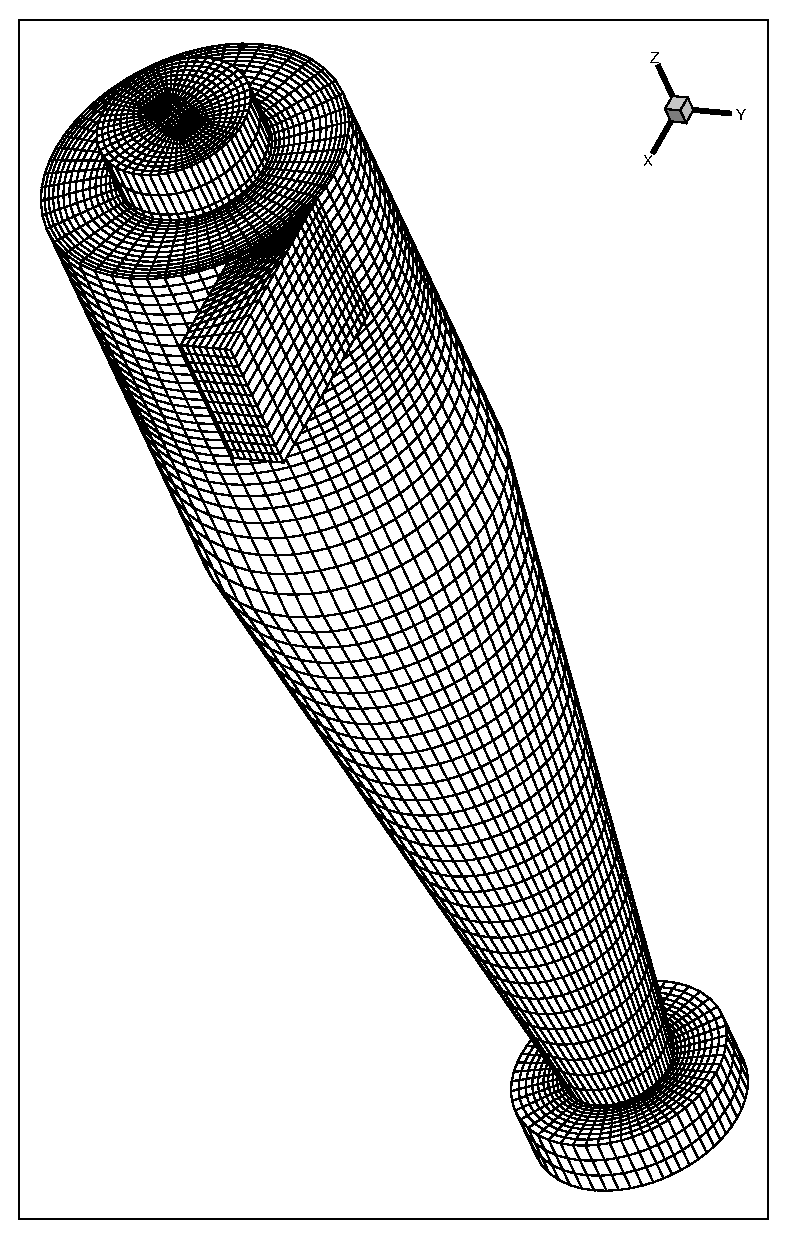
\includegraphics[scale=0.45]{meshCyclone}
	\captionof{figure}{Сетка расчётной области}
	\label{fig:cycloneMesh}
\end{minipage}
\vspace{1em}  
  \paragraph{Методические исследования\\}
  \addcontentsline{toc}{paragraph}{Методические исследования}

  Для исследования сеточной сходимости решения, расчёты задачи с  $U_{in} = 20m/s$ проводились на сетках 29380 ячеек, 96256 ячеек и 179552 ячейки. Сравнение профилей скорости вдоль двух отрезков, $1:$ $\left\{\left(0, 0, -0.3\right),\left(0.09, 0, -0,3\right)\right\}$ и $2:$ $\left\{\left(0, 0, -0.3\right),\left(0, 0.09, -0,3\right)\right\}$, представлены на \textit{рисунках \ref{fig:cycloneMeshIndependence1} -  \ref{fig:cycloneMeshIndependence4}}.
 \begin{figure}[h]
	\vspace{-1em}
	\begin{minipage}{0.475\linewidth}
		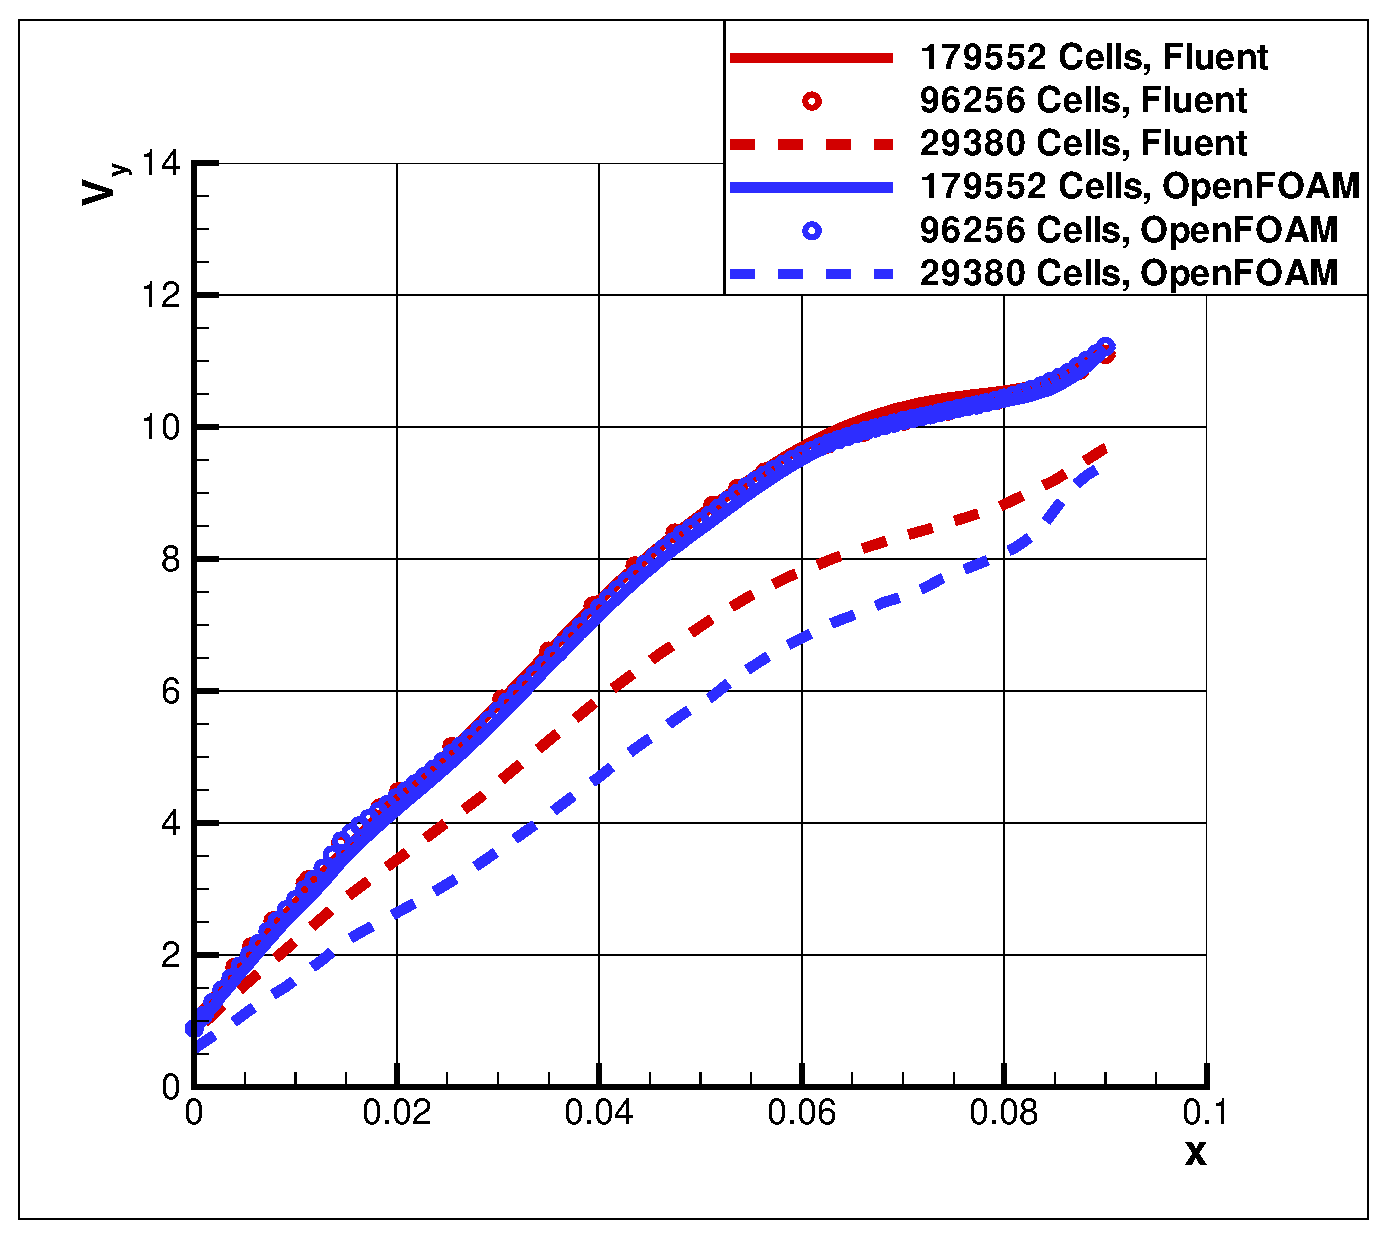
\includegraphics[scale=0.33]{cycloneMeshIndependence1}
		\caption{Профили $V_y$ вдоль прямой $1$}
		\label{fig:cycloneMeshIndependence1}
	\end{minipage}
	\hspace{0.5em}
	\begin{minipage}{0.475\linewidth}
		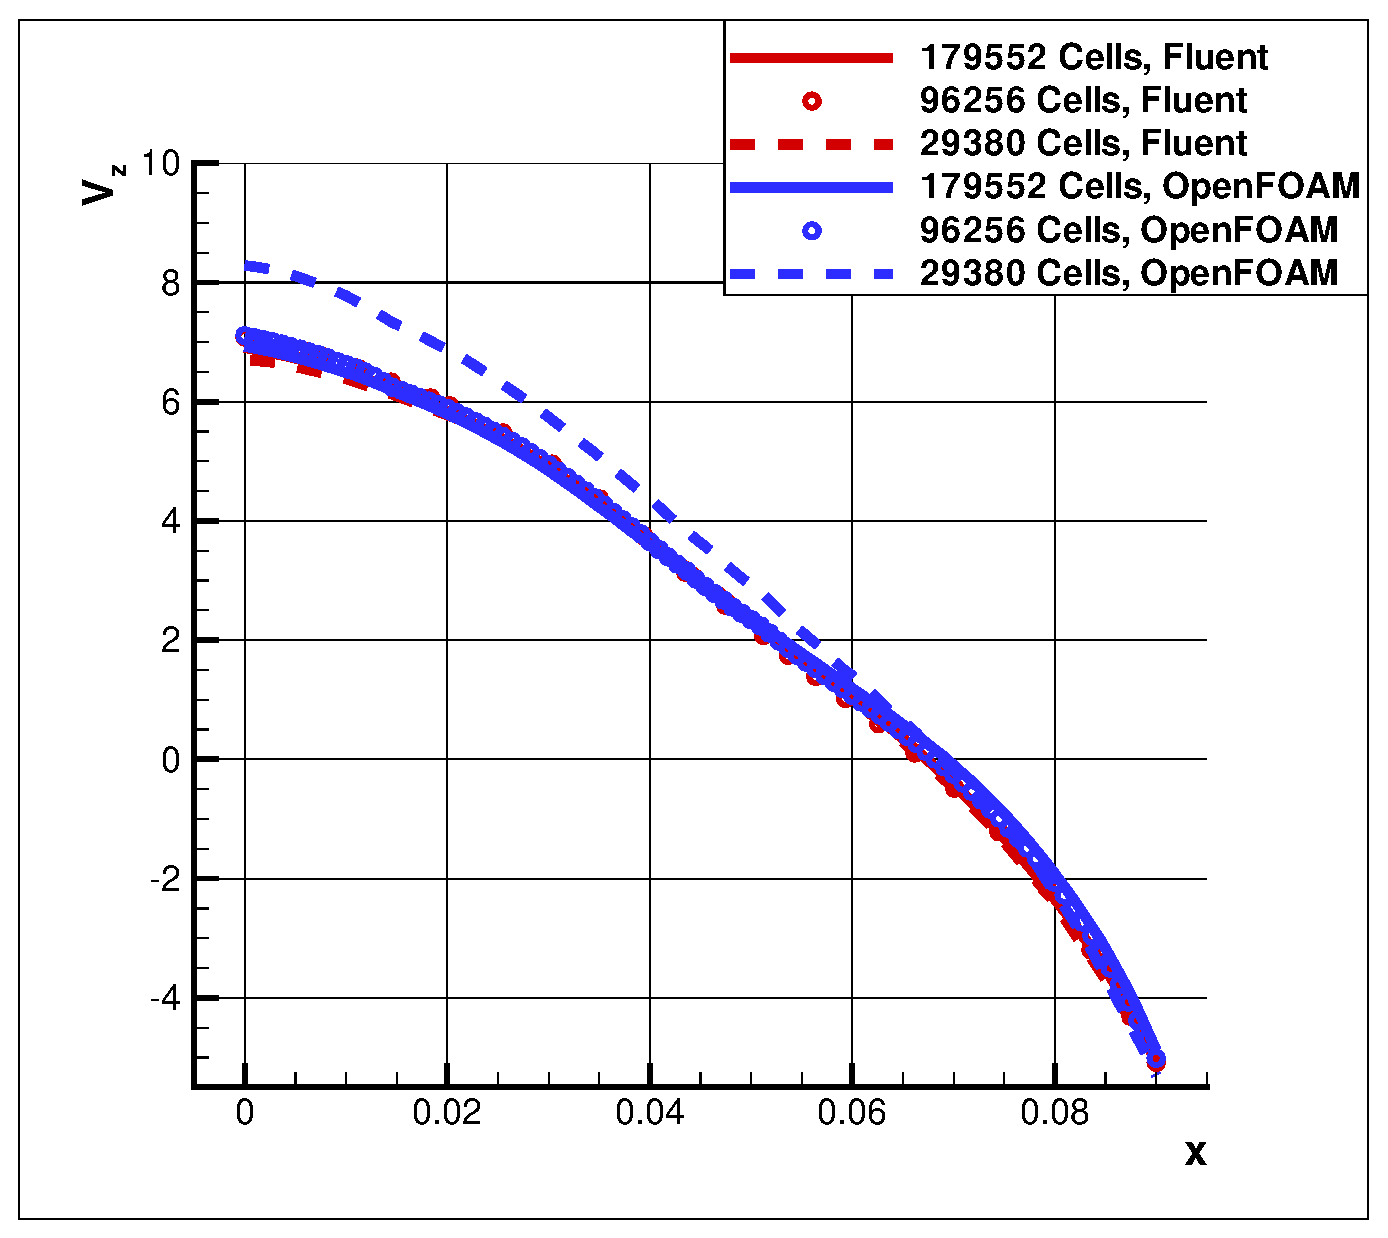
\includegraphics[scale=0.33]{cycloneMeshIndependence2}
		\caption{Профили $V_z$ вдоль прямой $1$}
		\label{fig:cycloneMeshIndependence2}
	\end{minipage}
\end{figure}

 \begin{figure}[h]
	\vspace{-1em}
	\begin{minipage}{0.475\linewidth}
		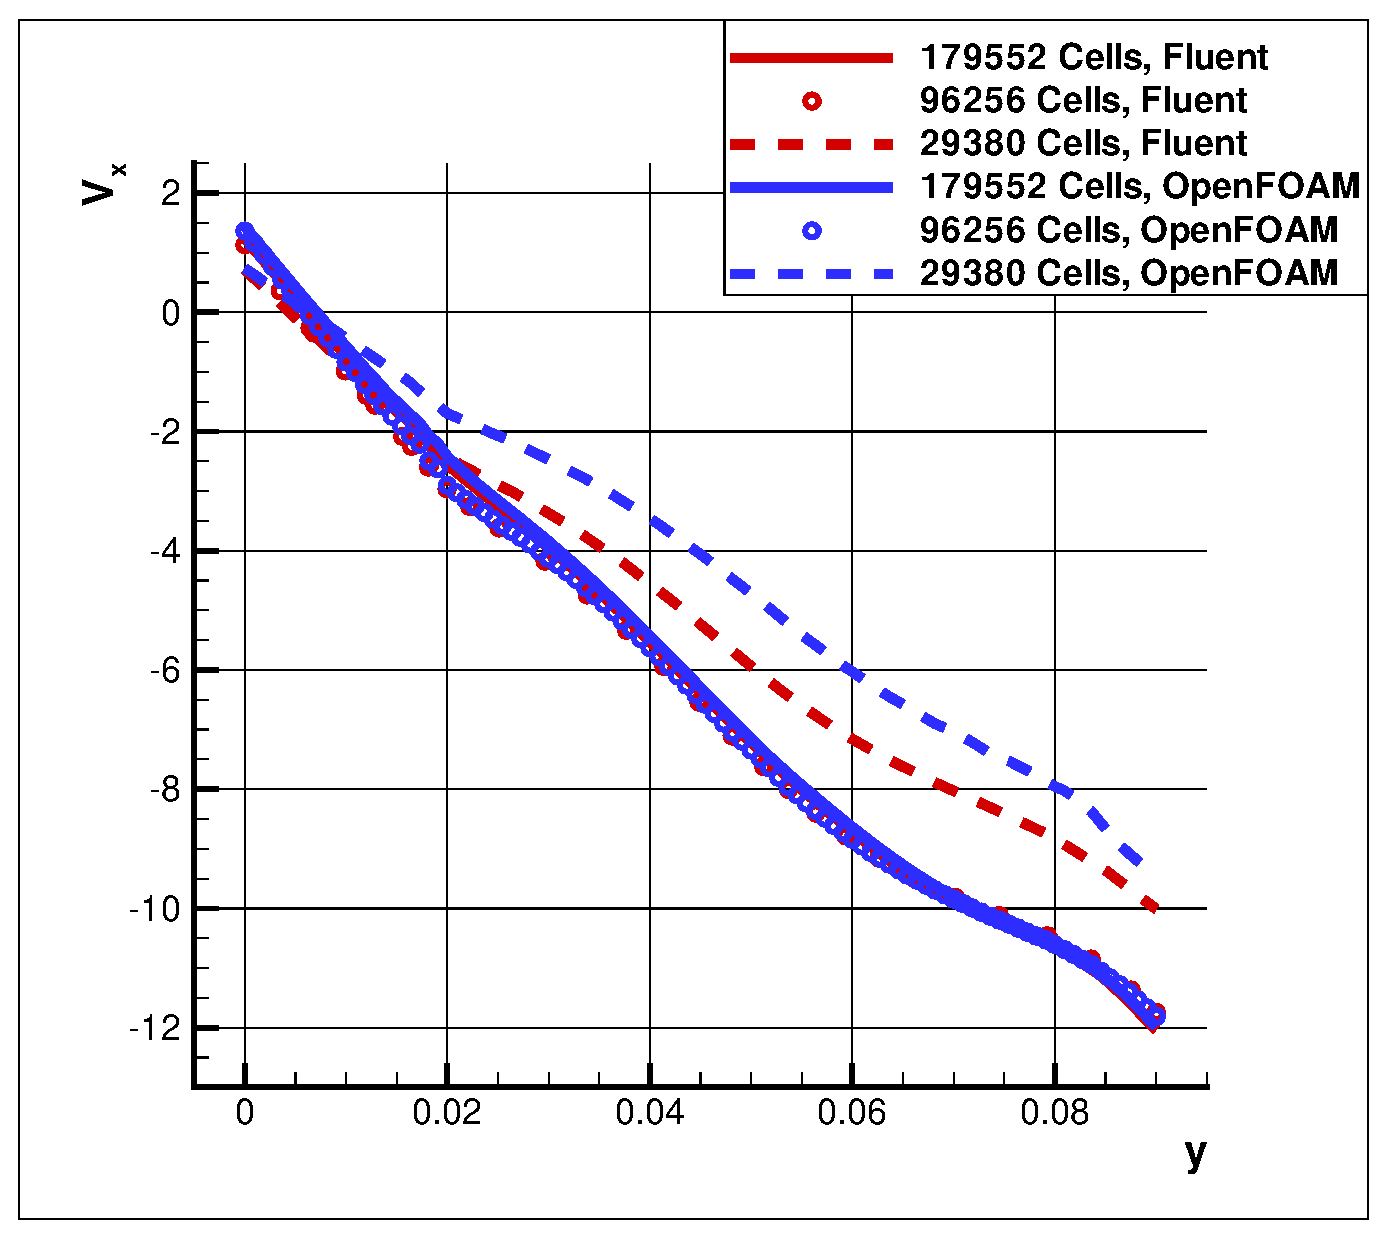
\includegraphics[scale=0.33]{cycloneMeshIndependence3}
		\caption{Профили $V_x$ вдоль прямой $2$}
		\label{fig:cycloneMeshIndependence3}
	\end{minipage}
	\hspace{0.5em}
	\begin{minipage}{0.475\linewidth}
		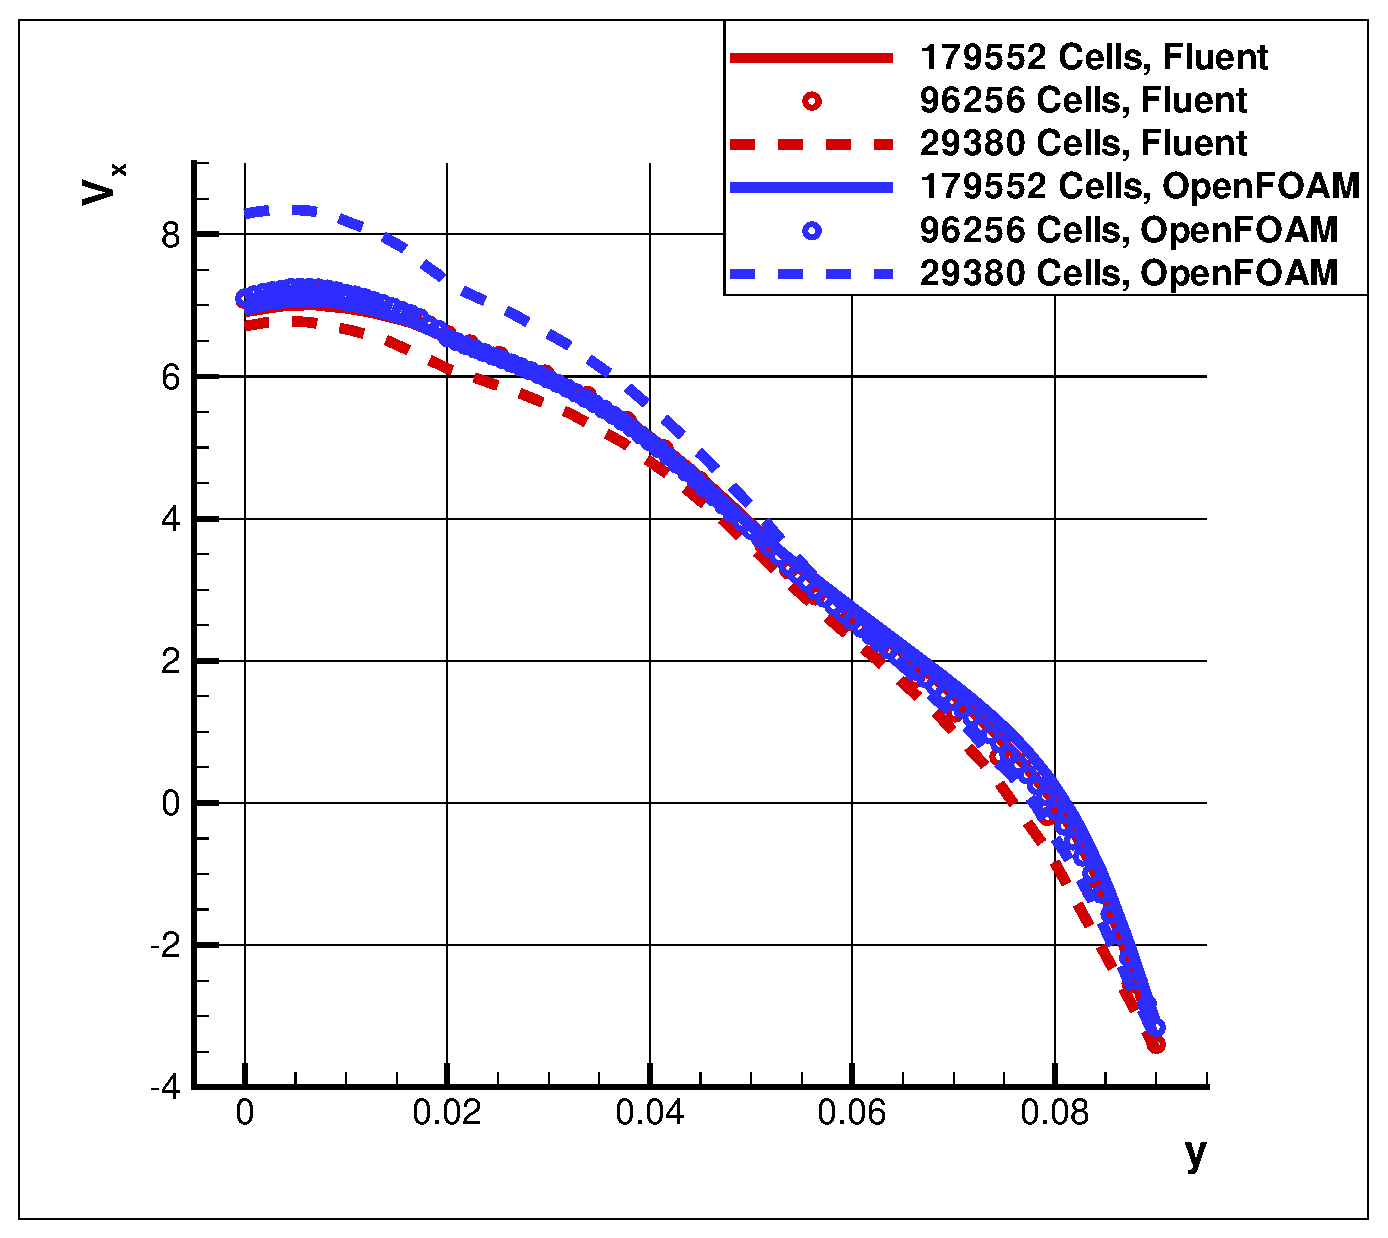
\includegraphics[scale=0.33]{cycloneMeshIndependence4}
		\caption{Профили $V_z$ вдоль прямой $2$}
		\label{fig:cycloneMeshIndependence4}
	\end{minipage}
\end{figure}
\clearpage
Видно, что решение на самой грубой сетке (29380 ячеек) сильно отличается от решения на более подробных сетках. В то же время, решение на сетках 96256 ячеек и 179552 ячейки отличаются менее, чем на 5\%, так что, сетки в 96256 ячеек вполне достаточно для получения сеточно-независимого решения. Кроме того, решения в Fluent и OpenFOAM хорошо соответствуют друг другу -- профили скорости на \textit{рисунках \ref{fig:cycloneMeshIndependence1} -  \ref{fig:cycloneMeshIndependence4}} для Fluent и OpenFOAM практически неотличимы для подробных сеток.

\begin{figure}[h]
	\centering
	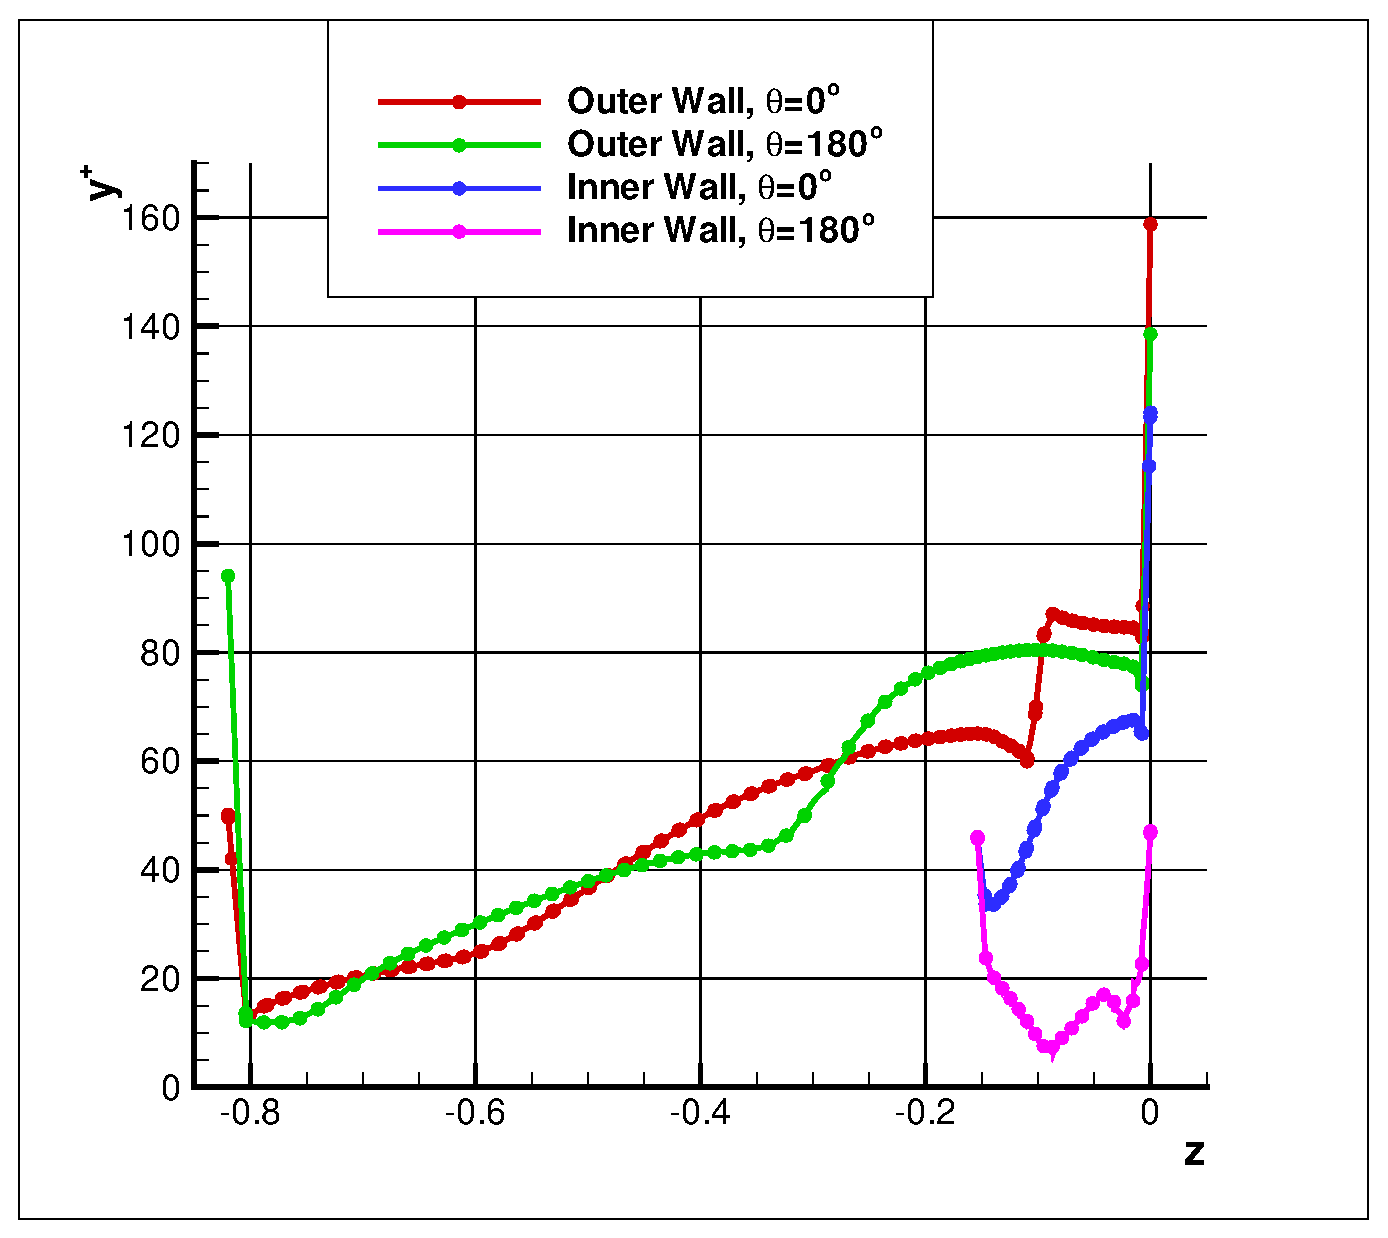
\includegraphics[scale=0.4]{yplusCyclone}
	\caption{Величина $y^{+}$ первой пристенной ячейки на внешней и внутренней стенках циклона}
	\label{fig:cycloneyPlus}
\end{figure}

На \textit{рисунке \ref{fig:cycloneyPlus}}, проиллюстрировано распределение величины $y^{+}$ первой пристенной ячейки, построенное вдоль образующих внешних и внутренных стенок, для углов $\theta=0^o$ и $\theta=180^o$ (отмечены на \textit{рисунке \ref{fig:cycloneGeometryScheme}} пунктирными линиями). Из графиков видно, что в большей части области величина $y^{+}$ лежит в пределах $10 \div 90$, что вполне адекватно для использования модели Ментера с автоматическими пристеночными функциями.

Решение, полученное с использованием OpenFOAM достаточно хорошо согласуется с решением, полученным в Fluent как для стандартной модели Ментера, так и для модели с поправкой на кривизну линий тока, что можно видеть по сопоставленным на \textit{рисунках \ref{fig:axialCyclone} - \ref{fig:tangentialCyclone2}} распределениям безразмерных осевой и тангенциальной составляющих скорости. Влияние поправки, как видно из первых двух рисунков, особенно сильно сказывается на течении вдоль выпуклых стенок выходной трубы. Такого результата и следовало ожидать в силу того, что немодифицированная модель Ментера занижает генерацию турбулентности в этой области. Видно также, что решение с использованием поправки несколько изменило профили скорости вблизи границы ядра циклона и в его центре.


Расчёт течения при наличии частиц в циклоне (как, собственно, и предыдущие расчёты) выполнен с использованием имплементированного в OpenFOAM солвера, учитывающего влияние дисперсных включений на несущую фазу. Надо сказать, что анализ результатов \textit{(рисунок \ref{fig:parcelsInteraction})} показал, что для рассматриваемой задачи дисперсные включения слабо влияют на основной поток.

\newpage
 \begin{figure}[h]
	\begin{minipage}{0.475\linewidth}
		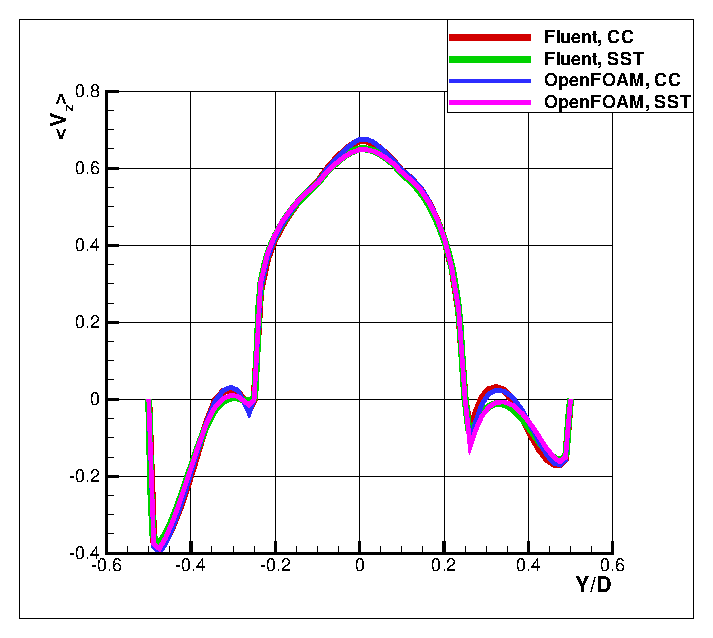
\includegraphics[scale=0.66]{axialCyclone}
		\caption{Профили $<V_{z}>$ вдоль прямой $Z/D=-0.75, x=0$}
		\label{fig:axialCyclone}
	\end{minipage}
	\hspace{0.5em}
	\begin{minipage}{0.475\linewidth}
		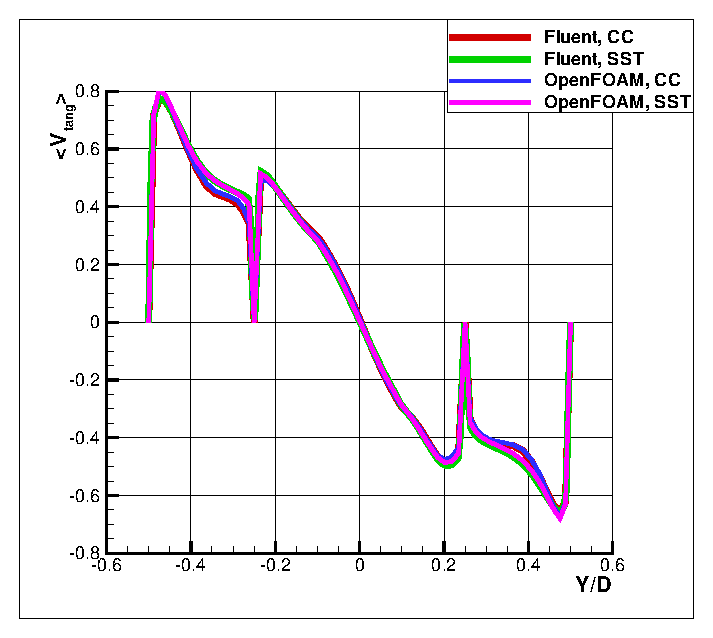
\includegraphics[scale=0.66]{tangentialCyclone}
		\caption{Профили $<V_{tang}>$ вдоль пр. $Z/D=-0.75, x=0$}
		\label{fig:tangentialCyclone}
	\end{minipage}
	\begin{minipage}{0.475\linewidth}
		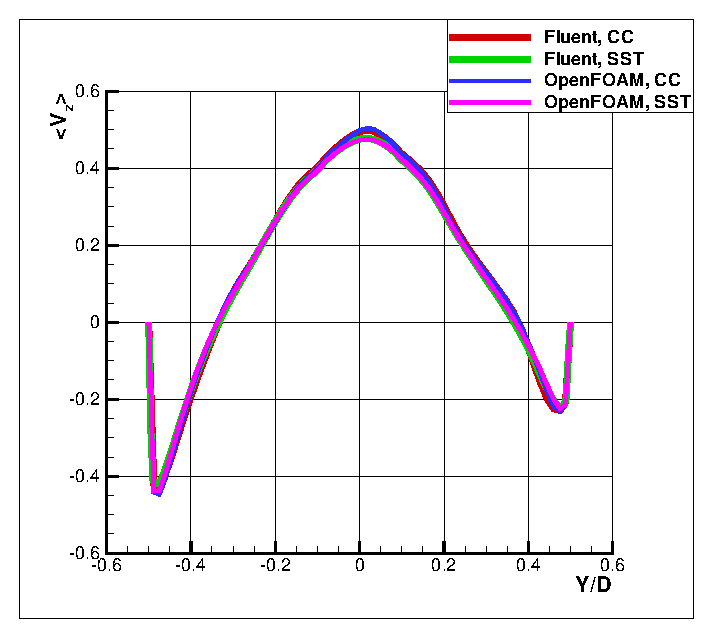
\includegraphics[scale=0.66]{axialCyclone2}
		\caption{Профили $<V_{z}>$ вдоль прямой $Z/D=-1, x=0$}
		\label{fig:axialCyclone2}
	\end{minipage}
	\hspace{0.5em}
	\begin{minipage}{0.475\linewidth}
		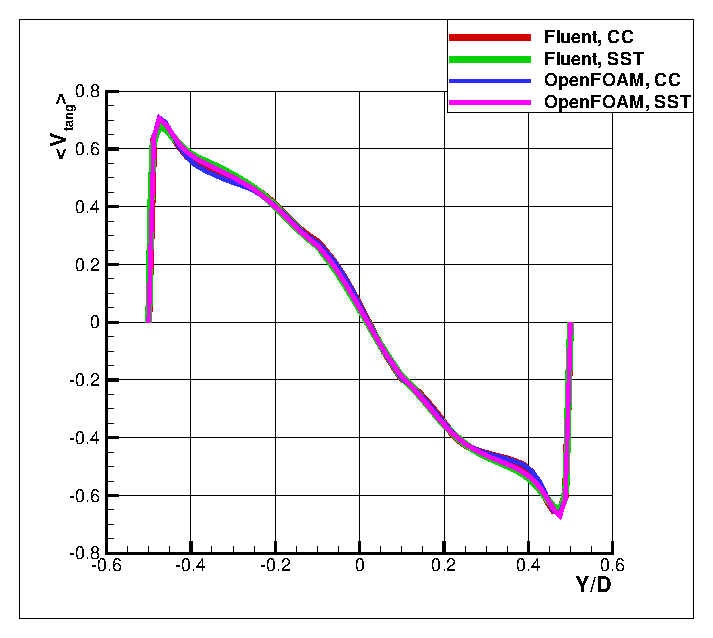
\includegraphics[scale=0.66]{tangentialCyclone2}
		\caption{Профили $<V_{tang}>$ вдоль пр. $Z/D=-1, x=0$}
		\label{fig:tangentialCyclone2}
	\end{minipage}
\end{figure}
\clearpage

\paragraph{Исследование эффективности циклона\\}
\addcontentsline{toc}{paragraph}{Исследование эффективности циклона}

На \textit{рисунках \ref{fig:parcelsCyclone1}-\ref{fig:parcelsCyclone4}} показано распределение частиц в циклоне для разных диаметров частиц и разных входных скоростей потока через секунду после запуска. За это время в циклон поступило, при различных условиях задачи, от одного миллиона до двух миллионов частиц. По интенсивности распределения частиц в выходной трубе можно судить, что эффективность для частиц диаметром порядка $10^{-5}m$ практически 100\%, для частиц диаметром $\sim 10^{-6}m$ она несколько меньше, а частицы диаметром $\sim 10^{-7}m$ в очень большом количестве вылетают из циклона. Кроме того, на \textit{рисункe \ref{fig:t1}} показано распределение частиц диаметром $\sim 10^{-6}m$ в циклоне для 10 моментов времени.

Эффективность, рассчитанная из отношения количества вылетевших и запущенных частиц в численном эксперименте, для различных параметров представлена в сравнении с экспериментальными данными Диргоу и Лейта \cite{DirgoLeith} в \textit{таблице \ref{tableSolution}}.

\begin{center}
	\begin{table}[h]
		\vspace{-1em}
		\caption{Результаты для эффективности циклонов}
		\label{tableSolution}
		\begin{tabular}{|c|c|c|}
			\hline
			Параметры течения & $\eta$, численное исследование & $\eta$, эксперимент \\
			\hline
			$U_{in}=20m/s, d=5 \cdot 10^{-5}m$ & 100\% & 100\% \\
			\hline
			$U_{in}=20m/s, d=5 \cdot 10^{-6}m$ & 93\% & 90\%\\
			\hline
			$U_{in}=20m/s, d=5 \cdot 10^{-7}m$ & 27\% & 10\%\\
			\hline
			$U_{in}=15m/s, d=10^{-5}m$ & 80\% & 90\% \\
			\hline
			$U_{in}=10m/s, d=10^{-5}m$ & 72\% & 85\% \\
			\hline
			$U_{in}=5m/s, d=10^{-5}m$ & 75\% & 80\% \\
			\hline
		\end{tabular}
	\end{table}
\end{center}
\clearpage
\begin{figure}[h]
 	\vspace{-4em}
	\begin{minipage}{0.475\linewidth}
		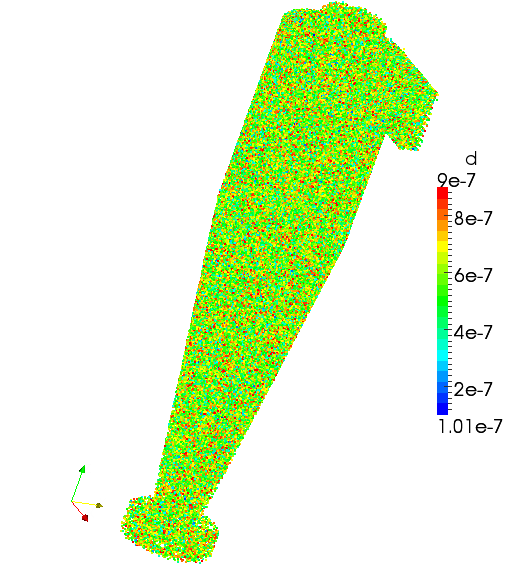
\includegraphics[scale=0.4]{parcelsCyclone1}
		\caption{Распределение частиц в циклоне для $d \sim 10^{-7}$ и $U_{in} = 20m/s$}
		\label{fig:parcelsCyclone1}
	\end{minipage}
	\hspace{0.5em}
	\begin{minipage}{0.475\linewidth}
		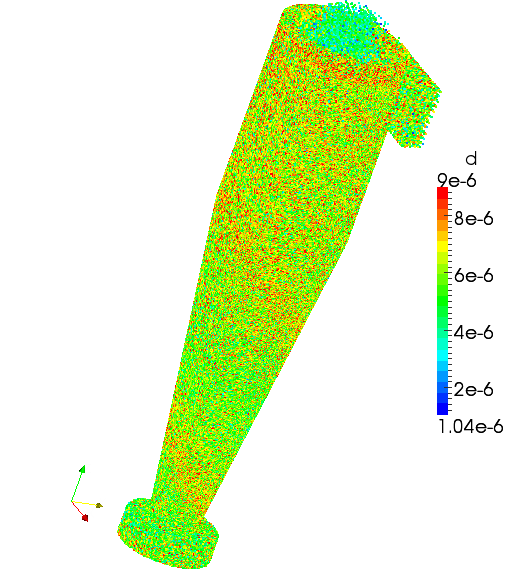
\includegraphics[scale=0.4]{parcelsCyclone2}
		\caption{Распределение частиц в циклоне для $d \sim 10^{-6}$ и $U_{in} = 20m/s$}
		\label{fig:parcelsCyclone2}
	\end{minipage}
	\begin{minipage}{0.475\linewidth}
		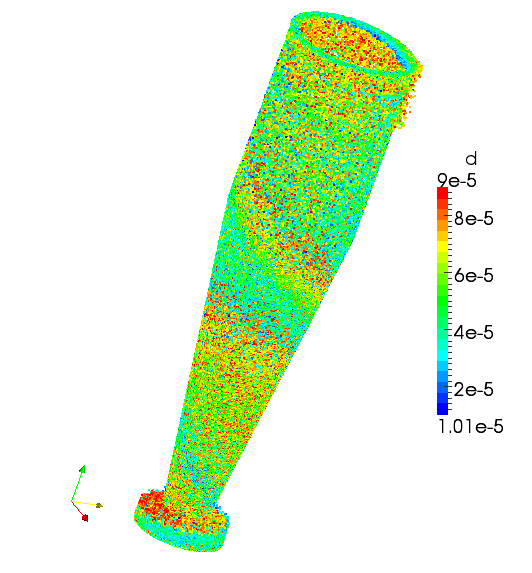
\includegraphics[scale=0.4]{parcelsCyclone3}
		\caption{Распределение частиц в циклоне для $d \sim 10^{-5}$ и $U_{in} = 20m/s$}
		\label{fig:parcelsCyclone3}
	\end{minipage}
	\hspace{0.5em}
	\begin{minipage}{0.475\linewidth}
		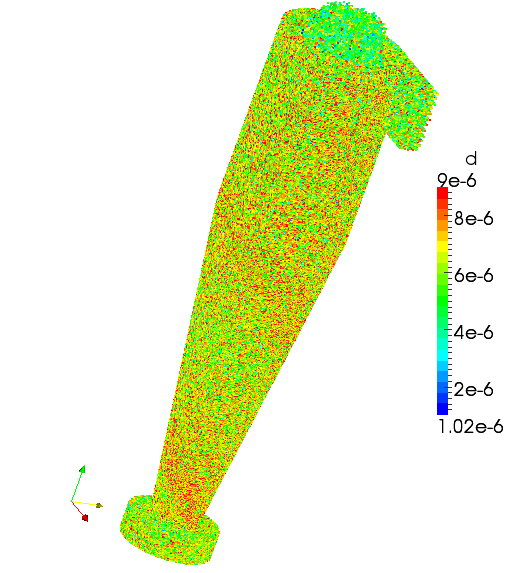
\includegraphics[scale=0.4]{parcelsCyclone4}
		\caption{Распределение частиц в циклоне для $d \sim 10^{-5}$ и $U_{in} = 10m/s$}
		\label{fig:parcelsCyclone4}
	\end{minipage}
\end{figure}
\clearpage
 \begin{figure}[h]
 	\centering
 	\vspace{-4em}
 	\hspace{-1em}
	\begin{minipage}{0.2\linewidth}
		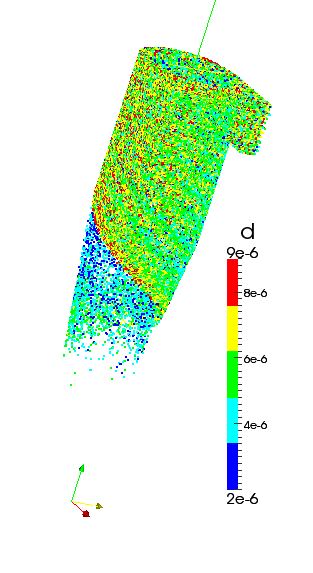
\includegraphics[scale=0.3]{t1}
		\text{t=0.1s}
	\end{minipage}
	\hspace{-1em}
	\begin{minipage}{0.2\linewidth}
		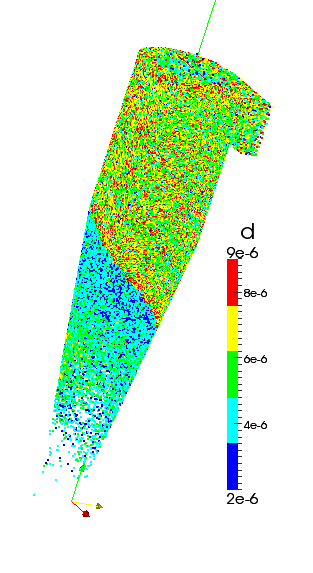
\includegraphics[scale=0.3]{t2}
		\text{t=0.2s}
	\end{minipage}
		\hspace{-1em}
	\begin{minipage}{0.2\linewidth}
		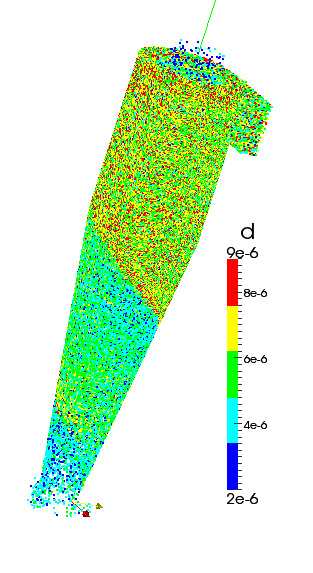
\includegraphics[scale=0.3]{t3}
		\text{t=0.3s}
	\end{minipage}
		\hspace{-1em}
	\begin{minipage}{0.2\linewidth}
		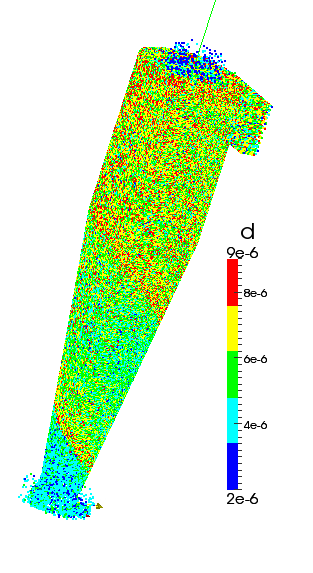
\includegraphics[scale=0.3]{t4}
		\text{t=0.4s}
	\end{minipage}
		\hspace{-1em}
	\begin{minipage}{0.2\linewidth}
		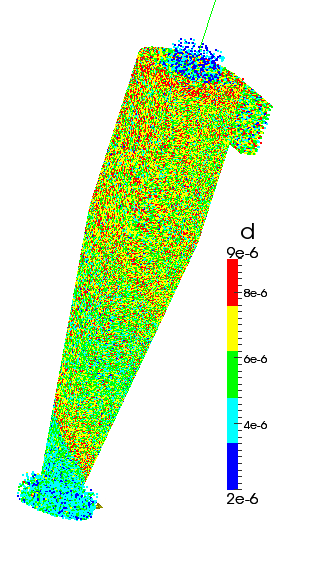
\includegraphics[scale=0.3]{t5}
		\text{t=0.5s}
	\end{minipage}
		\hspace{-1em}
	\begin{minipage}{0.2\linewidth}
		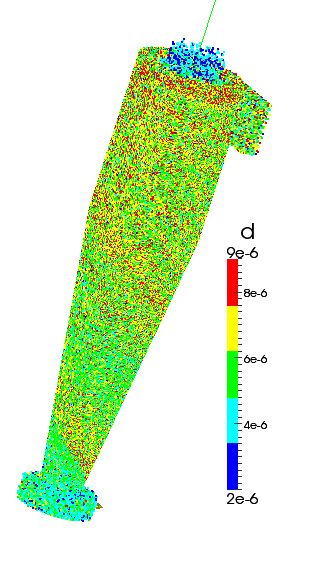
\includegraphics[scale=0.3]{t6}
		\text{t=0.6s}
	\end{minipage}
		\hspace{-1em}
	\begin{minipage}{0.2\linewidth}
		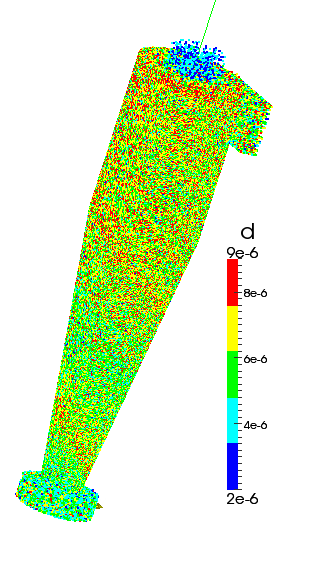
\includegraphics[scale=0.3]{t7}
		\text{t=0.7s}
	\end{minipage}
		\hspace{-1em}
	\begin{minipage}{0.2\linewidth}
		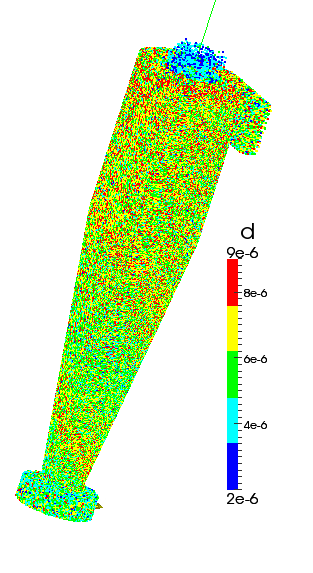
\includegraphics[scale=0.3]{t8}
		\text{t=0.8s}
	\end{minipage}
		\hspace{-1em}
	\begin{minipage}{0.2\linewidth}
		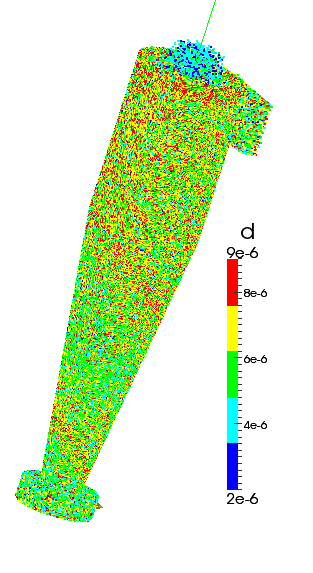
\includegraphics[scale=0.3]{t9}
		\text{t=0.9s}
	\end{minipage}
		\hspace{-1em}
	\begin{minipage}{0.2\linewidth}
		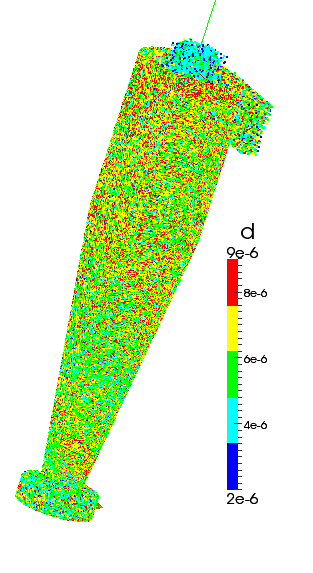
\includegraphics[scale=0.3]{t10}
		\text{t=1s}
	\end{minipage}
	\captionof{figure}{Развитие течения дисперсных включений}
	\label{fig:t1}
\end{figure}
Из \textit{таблицы \ref{tableSolution}} видно, что полученные с использованием написанного солвера результаты достаточно хорошо согласуются с экспериментальными данными Диргоу и Лейта для степени очистки.

Очевидно, при уменьшении диаметра частиц, эффективность циклонов падает. При диаметре $ \sim 10^{-7}m$ почти три четверти частиц вылетают через выходную трубу вместе с потоком. При уменьшении скорости, эффективность фильтра так же падает, так как уменьшается центробежная сила, и, следовательно, частицы медленнее относятся к стенке и не отсоединяются от основного потока. При уменьшении скорости график зависимости степени очистки от диаметра частиц смещается в сторону больших диаметров, что подтверждается как теорией и экспериментами, так и численными расчётами.

Описанные выше результаты говорят в пользу правильности имплементированного в OpenFOAM солвера, позволяющего рассчитывать турбулентные течения сжимаемого теплопроводящего газа с учётом обратного влияния частиц на основной поток.
\begin{figure}[h]
	\centering
	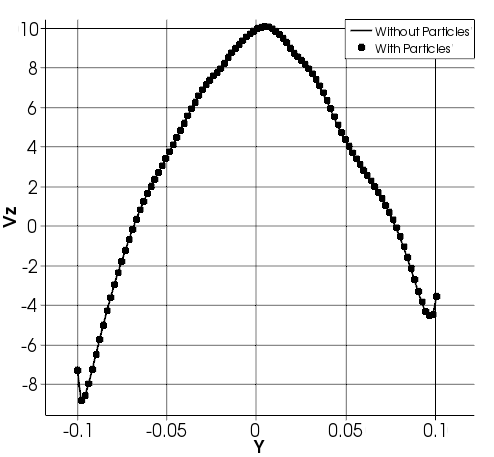
\includegraphics[scale=0.75]{parcelsInteraction}
	\caption{Влияние частиц на основное течение}
	\label{fig:parcelsInteraction}
\end{figure}